% Options for packages loaded elsewhere
\PassOptionsToPackage{unicode}{hyperref}
\PassOptionsToPackage{hyphens}{url}
%
\documentclass[
]{book}
\usepackage{lmodern}
\usepackage{amssymb,amsmath}
\usepackage{ifxetex,ifluatex}
\ifnum 0\ifxetex 1\fi\ifluatex 1\fi=0 % if pdftex
  \usepackage[T1]{fontenc}
  \usepackage[utf8]{inputenc}
  \usepackage{textcomp} % provide euro and other symbols
\else % if luatex or xetex
  \usepackage{unicode-math}
  \defaultfontfeatures{Scale=MatchLowercase}
  \defaultfontfeatures[\rmfamily]{Ligatures=TeX,Scale=1}
\fi
% Use upquote if available, for straight quotes in verbatim environments
\IfFileExists{upquote.sty}{\usepackage{upquote}}{}
\IfFileExists{microtype.sty}{% use microtype if available
  \usepackage[]{microtype}
  \UseMicrotypeSet[protrusion]{basicmath} % disable protrusion for tt fonts
}{}
\makeatletter
\@ifundefined{KOMAClassName}{% if non-KOMA class
  \IfFileExists{parskip.sty}{%
    \usepackage{parskip}
  }{% else
    \setlength{\parindent}{0pt}
    \setlength{\parskip}{6pt plus 2pt minus 1pt}}
}{% if KOMA class
  \KOMAoptions{parskip=half}}
\makeatother
\usepackage{xcolor}
\IfFileExists{xurl.sty}{\usepackage{xurl}}{} % add URL line breaks if available
\IfFileExists{bookmark.sty}{\usepackage{bookmark}}{\usepackage{hyperref}}
\hypersetup{
  pdftitle={CH10009 Workshop Questions},
  pdfauthor={Fiona Dickinson},
  hidelinks,
  pdfcreator={LaTeX via pandoc}}
\urlstyle{same} % disable monospaced font for URLs
\usepackage{longtable,booktabs}
% Correct order of tables after \paragraph or \subparagraph
\usepackage{etoolbox}
\makeatletter
\patchcmd\longtable{\par}{\if@noskipsec\mbox{}\fi\par}{}{}
\makeatother
% Allow footnotes in longtable head/foot
\IfFileExists{footnotehyper.sty}{\usepackage{footnotehyper}}{\usepackage{footnote}}
\makesavenoteenv{longtable}
\usepackage{graphicx,grffile}
\makeatletter
\def\maxwidth{\ifdim\Gin@nat@width>\linewidth\linewidth\else\Gin@nat@width\fi}
\def\maxheight{\ifdim\Gin@nat@height>\textheight\textheight\else\Gin@nat@height\fi}
\makeatother
% Scale images if necessary, so that they will not overflow the page
% margins by default, and it is still possible to overwrite the defaults
% using explicit options in \includegraphics[width, height, ...]{}
\setkeys{Gin}{width=\maxwidth,height=\maxheight,keepaspectratio}
% Set default figure placement to htbp
\makeatletter
\def\fps@figure{htbp}
\makeatother
\setlength{\emergencystretch}{3em} % prevent overfull lines
\providecommand{\tightlist}{%
  \setlength{\itemsep}{0pt}\setlength{\parskip}{0pt}}
\setcounter{secnumdepth}{5}
\usepackage{booktabs}
\usepackage{amsthm}
\makeatletter
\def\thm@space@setup{%
  \thm@preskip=8pt plus 2pt minus 4pt
  \thm@postskip=\thm@preskip
}
\makeatother
\usepackage[]{natbib}
\bibliographystyle{apalike}

\title{CH10009 Workshop Questions}
\author{Fiona Dickinson}
\date{2020-10-20}

\begin{document}
\maketitle

{
\setcounter{tocdepth}{1}
\tableofcontents
}
\hypertarget{welcome}{%
\chapter*{Welcome}\label{welcome}}
\addcontentsline{toc}{chapter}{Welcome}

The notes have been prepared in a package called BookDown for RStudio so that the equations are accessible to screen readers. However, by providing the notes as a .html webpage I can also embed short videos to further describe some of the topics. Further you can download the questions (and later the answers, top left of the screen) in a format that suits you (either pdf or epub) to view offline, or change the way this document appears for ease of reading.

If you spot any typos or think there are any errors please let me know and I will do my best to fix them.

\hypertarget{workshops-for-ch10009}{%
\section*{Workshops for CH10009}\label{workshops-for-ch10009}}
\addcontentsline{toc}{section}{Workshops for CH10009}

The topics for LOILS each week are as follows:

\begin{itemize}
\tightlist
\item
  Week 1: General Q\&A
\item
  Week 2: Rearranging equations, units and standard form
\item
  Week 3: Logarithms and exponentials
\item
  Week 4: Tables and graphs
\item
  Week 5: Calculus - differentiation - the basics and the chain rule
\item
  Week 6: Calculus - differentiation - the product rule and partial differentiation
\item
  Week 7: Calculus - integration - the basics and definite integrals
\item
  Week 8: Some more examples of integration and revision
\end{itemize}

This `book' will be updated weekly with workshop questions, answers will be provided and some answers will include `process' as well as answer. Please contact me if you need help.

I am using this format as it is an accessible format.

\hypertarget{version-history}{%
\section*{Version history}\label{version-history}}
\addcontentsline{toc}{section}{Version history}

Week 3 workshop released 19th October 2020

Week 2 workshop released 12th October 2020.

Some more video answers for workshop 1 embedded 11th October 2020.

Video answers for workshop 1 embedded 09th October 2020.

The initial commit of this book is dated 2nd October 2020.

\hypertarget{ch:Workshop1}{%
\chapter{Week 1}\label{ch:Workshop1}}

\hypertarget{sec:Prelim}{%
\section{Preliminary infomation}\label{sec:Prelim}}

\hypertarget{si-base-units}{%
\subsection{SI base units}\label{si-base-units}}

The SI system of base units has seven fundamental units from which the others are derived.

\begin{longtable}[]{@{}cccc@{}}
\caption{\label{tab:SIbase} The seven base units from which all others are dervied.}\tabularnewline
\toprule
SI base unit & symbol & quantity symbol (dimension) & quantity\tabularnewline
\midrule
\endfirsthead
\toprule
SI base unit & symbol & quantity symbol (dimension) & quantity\tabularnewline
\midrule
\endhead
kilogram & kg & M & mass\tabularnewline
metre & m & L & length\tabularnewline
second & s & T & time\tabularnewline
ampere & A & I & electric current\tabularnewline
kelvin & K & Θ & temperature\tabularnewline
mole & mol & N & amount of substance\tabularnewline
candela & cd & J & luminous intensity\tabularnewline
\bottomrule
\end{longtable}

\hypertarget{si-derived-units}{%
\subsection{SI Derived units}\label{si-derived-units}}

\begin{longtable}[]{@{}ccccc@{}}
\caption{\label{tab:SIderive} Some common SI derived units used in chemistry.}\tabularnewline
\toprule
symbol & SI derived unit & quantity & SI base units & other SI units\tabularnewline
\midrule
\endfirsthead
\toprule
symbol & SI derived unit & quantity & SI base units & other SI units\tabularnewline
\midrule
\endhead
Hz & hertz & frequency & s\textsuperscript{-1} &\tabularnewline
N & newton & force & kg m s\textsuperscript{-2} &\tabularnewline
Pa & pascal & pressure & kg m\textsuperscript{-1} s\textsuperscript{-2} & N m\textsuperscript{-2}\tabularnewline
J & joule & energy & kg m\textsuperscript{2} s\textsuperscript{-2} & N m\tabularnewline
W & watt & power & kg m\textsuperscript{2} s\textsuperscript{-3} & J s\textsuperscript{-1}\tabularnewline
C & coulomb & electrical charge & A s &\tabularnewline
V & volt & electrical potential & kg m\textsuperscript{2} s\textsuperscript{-3} A\textsuperscript{-1} & J C\textsuperscript{-1}\tabularnewline
F & farad & electrical capacitance & kg\textsuperscript{-1} m\textsuperscript{-2} s\textsuperscript{4} A\textsuperscript{2} & C V\textsuperscript{-1}\tabularnewline
Ω & ohm & electrical resistance & kg m\textsuperscript{2} s\textsuperscript{-3} A\textsuperscript{-2} & V A\textsuperscript{-1}\tabularnewline
S & siemens & electrical conductance & kg\textsuperscript{-1} m\textsuperscript{-2} s\textsuperscript{3} A\textsuperscript{2} & A V\textsuperscript{-1} or 1/Ω\tabularnewline
\bottomrule
\end{longtable}

\hypertarget{other-units-and-conversion-factors}{%
\subsection{Other units and conversion factors}\label{other-units-and-conversion-factors}}

There are a number of non-SI base or derived units which are in common usage which are useful to know and be able to convert between. Table \ref{tab:nonSI} contains a number of useful unit conversions.

\begin{longtable}[]{@{}ccc@{}}
\caption{\label{tab:nonSI} The relationship between some other common units and the SI system.}\tabularnewline
\toprule
unit & quantity & SI equivalant\tabularnewline
\midrule
\endfirsthead
\toprule
unit & quantity & SI equivalant\tabularnewline
\midrule
\endhead
torr (or mm Hg) & pressure & \(\frac{101325}{760}\) Pa\tabularnewline
atm & pressure & 101325 Pa\tabularnewline
bar & pressure & 100000 Pa\tabularnewline
eV & energy & 1.602176634 × 10\textsuperscript{-19} J\tabularnewline
cal & energy & 4.184 J\tabularnewline
Å & length & 1 × 10\textsuperscript{-10} m\tabularnewline
\bottomrule
\end{longtable}

There are myriad other units in use, either with historical or geographic preference, or just for niche purposes (where would we be without olympic swimming pools or London buses). Examples such as the mile, furlong or beard-second are all units of length.

Further, the unit ºC is formally an SI derived unit. The temperature in Kelvin is:

\begin{equation*}
T (\textrm{K}) = T (\textrm{K}) + 273.15
\end{equation*}

\hypertarget{si-prefixes-and-standard-form}{%
\subsection{SI prefixes and standard form}\label{si-prefixes-and-standard-form}}

In general lower case prefixes are used for negative powers and upper case prefixes are used for positive powers, however k (kilo) is an obvious exception to this rule. (Other exceptions are da (deca, 10\textsuperscript{1}) and h (hecto, 10\textsuperscript{2})).

\begin{longtable}[]{@{}ccc@{}}
\caption{\label{tab:SIprefix} The more common SI prefixes used in chemistry.}\tabularnewline
\toprule
SI prefix & SI prefix `name' & standard form multiplier\tabularnewline
\midrule
\endfirsthead
\toprule
SI prefix & SI prefix `name' & standard form multiplier\tabularnewline
\midrule
\endhead
y & yocto & 10\textsuperscript{-24}\tabularnewline
z & zepto & 10\textsuperscript{-21}\tabularnewline
a & atto & 10\textsuperscript{-18}\tabularnewline
f & femto & 10\textsuperscript{-15}\tabularnewline
p & pico & 10\textsuperscript{-12}\tabularnewline
n & nano & 10\textsuperscript{-9}\tabularnewline
μ & micro & 10\textsuperscript{-6}\tabularnewline
m & milli & 10\textsuperscript{-3}\tabularnewline
c & centi & 10\textsuperscript{-2}\tabularnewline
d & deci & 10\textsuperscript{-1}\tabularnewline
& &\tabularnewline
k & kilo & 10\textsuperscript{3}\tabularnewline
\bottomrule
\end{longtable}

\hypertarget{sec:Questions}{%
\section{Questions}\label{sec:Questions}}

\hypertarget{subsec:rearrange}{%
\subsection{Rearranging equations}\label{subsec:rearrange}}

Answers for these questions are in Section \ref{subsec:rearrangeans}.

For each of the following rearrange to make the specified variable the subject of the equation.

\begin{enumerate}
\def\labelenumi{\arabic{enumi}.}
\tightlist
\item
  \([A]= [A]_0 - kt\), \(t\)
\item
  \(E = \frac{1}{2}mv^2\), \(v\)
\item
  \(F = \frac{q_1 q_2}{4 \pi \varepsilon _0 r^2}\), \(r\)
\item
  \(\frac{1}{[A]}=\frac{1}{[A]_0}+kt\), \([A]_0\)
\item
  \(\ln (x_A)=-\frac{\Delta H}{R}(\frac{1}{T_1}-\frac{1}{T_2})\), \(T_1\)
\item
  \(K_a=\frac{\alpha ^2 c}{1- \alpha}\), \(\alpha\)
\end{enumerate}

\hypertarget{subsec:Unitconv}{%
\subsection{Unit conversion questions}\label{subsec:Unitconv}}

Answers for these questions are in Section \ref{subsec:Unitconvans}.

\begin{enumerate}
\def\labelenumi{\arabic{enumi}.}
\tightlist
\item
  Convert the following:

  \begin{enumerate}
  \def\labelenumii{\alph{enumii}.}
  \tightlist
  \item
    3.4 µm to mm and m
  \item
    270.4 g mol\textsuperscript{-1} to kg mol\textsuperscript{-1} and yg (molecule\textsuperscript{-1})
  \item
    23.4 μg dm\textsuperscript{−3} to mg dm\textsuperscript{−3}, g m\textsuperscript{−3}, and kg m\textsuperscript{−3}
  \item
    17.5 µHz to Hz
  \item
    5796 cm\textsuperscript{-1} to µm\textsuperscript{-1} and m\textsuperscript{-1}
  \end{enumerate}
\end{enumerate}

\begin{center}\rule{0.5\linewidth}{0.5pt}\end{center}

\begin{enumerate}
\def\labelenumi{\arabic{enumi}.}
\setcounter{enumi}{1}
\tightlist
\item
  If a box has dimensions 0.234 m x 34.5 cm x 26.8 mm. What is the volume of the box in:

  \begin{enumerate}
  \def\labelenumii{\alph{enumii}.}
  \tightlist
  \item
    cm\textsuperscript{3}?
  \item
    dm\textsuperscript{3}?
  \item
    m\textsuperscript{3}?
  \item
    Å\textsuperscript{3}?
  \end{enumerate}
\end{enumerate}

\begin{center}\rule{0.5\linewidth}{0.5pt}\end{center}

\begin{enumerate}
\def\labelenumi{\arabic{enumi}.}
\setcounter{enumi}{2}
\tightlist
\item
  The Gibbs free energy of a reaction, \(\Delta G\) is given by equation \eqref{eq:gibbs}.
\end{enumerate}

\begin{equation}
\Delta G = \Delta H - T \Delta S
\label{eq:gibbs}
\end{equation}

Determine the value of \(\Delta G\) at 40 ºC when the enthalpy of reaction, \(\Delta H\) = -10.235 kJ mol\textsuperscript{-1} and the molar entropy, \(\Delta S\) = +34 J K\textsuperscript{-1} mol\textsuperscript{-1}

\hypertarget{subsec:detunits}{%
\subsection{Determining units of variables in equations}\label{subsec:detunits}}

Answers for these questions are in Section \ref{subsec:detunitsans}.

\begin{enumerate}
\def\labelenumi{\arabic{enumi}.}
\tightlist
\item
  The ideal gas equation is given in equation \eqref{eq:idealgas}.
\end{enumerate}

\begin{equation}
pV = n\textrm{R}T
\label{eq:idealgas}
\end{equation}

The units of the variables are:
\(p\) (pressure), Pa (pascals)
\(V\) (volume), m\textsuperscript{3}
\(n\) (number of moles), mol
\(T\) (absolute temperature), K

\begin{enumerate}
\def\labelenumi{\alph{enumi}.}
\item
  Determine the SI base units of the gas constant, R.
\item
  Determine the pressure in mmHg of 1.00 mmol of an ideal gas that occupies 1.65 dm\textsuperscript{3} at 25 ºC.
\end{enumerate}

\begin{center}\rule{0.5\linewidth}{0.5pt}\end{center}

\begin{enumerate}
\def\labelenumi{\arabic{enumi}.}
\setcounter{enumi}{1}
\tightlist
\item
  The famous Einstein equation \(E=mc^2\) is more properly written as:
\end{enumerate}

\begin{equation*}
E^2 = p^2 c^2 + m_0^2 c^4
\end{equation*}

Determine the units of the variable \(p\).

\begin{center}\rule{0.5\linewidth}{0.5pt}\end{center}

\begin{enumerate}
\def\labelenumi{\arabic{enumi}.}
\setcounter{enumi}{2}
\tightlist
\item
  At low temperatures the molar heat capacity of a material \(C_{p, m}\) (J K\textsuperscript{-1} mol\textsuperscript{-1}) is given by equation \eqref{eq:lowtempheat}.
\end{enumerate}

\begin{equation}
C_{p, m}= a T^3
\label{eq:lowtempheat}
\end{equation}

Determine the units of the constant, a.

\begin{center}\rule{0.5\linewidth}{0.5pt}\end{center}

\begin{enumerate}
\def\labelenumi{\arabic{enumi}.}
\setcounter{enumi}{3}
\tightlist
\item
  Determine the units of the coulomb constant, \(k_e\), in equation \eqref{eq:coulomb}, given that r is the separation of two charges, F the force of attraction between the two charges, and \(q_x\) is the charge (in coulombs, C) on each of the particles.
\end{enumerate}

\begin{equation}
F = k_e \frac{q_1 q_2}{r^2}
\label{eq:coulomb}
\end{equation}

\hypertarget{sec:Answers}{%
\section{Answers}\label{sec:Answers}}

\hypertarget{subsec:rearrangeans}{%
\subsection{Rearranging equations answers}\label{subsec:rearrangeans}}

\begin{enumerate}
\def\labelenumi{\arabic{enumi}.}
\tightlist
\item
  \(t =\frac{[A]_0-[A]}{k}\)
\item
  \(v = \sqrt {\frac{2E}{m}}\)
\item
  \(r = \sqrt{\frac{q_1 q_2}{4 \pi \varepsilon_0 F }}\)
\item
  \([A]_0=\frac{[A]}{1-[A]kt}\)
\item
  \(\frac{\Delta H T_2}{\Delta H - R T \ln {x_A}}\)
\end{enumerate}

\begin{enumerate}
\def\labelenumi{\arabic{enumi}.}
\tightlist
\item
  \(\alpha = \frac{-K_a \pm \sqrt{K_a^2 + 4 c K_a}}{2c}\)
\end{enumerate}

\hypertarget{subsec:Unitconvans}{%
\subsection{Unit conversion answers}\label{subsec:Unitconvans}}

\begin{enumerate}
\def\labelenumi{\arabic{enumi}.}
\item
  \begin{enumerate}
  \def\labelenumii{\alph{enumii}.}
  \tightlist
  \item
    3.4 × 10\textsuperscript{-3} mm; 3.4 × 10\textsuperscript{-6} m
  \item
    0.2704 kg mol\textsuperscript{-1}; 449.0 yg
  \end{enumerate}

  \begin{enumerate}
  \def\labelenumii{\alph{enumii}.}
  \setcounter{enumii}{2}
  \tightlist
  \item
    23.4 × 10\textsuperscript{-3} mg dm\textsuperscript{−3}; 23.4 × 10\textsuperscript{-3} g m\textsuperscript{−3}; and 23.4 × 10\textsuperscript{-6} kg m\textsuperscript{−3}
  \item
    17.5 × 10\textsuperscript{-6} Hz
  \item
    0.5796 µm\textsuperscript{-1} and 5.796 × 10\textsuperscript{5} m\textsuperscript{-1}
  \end{enumerate}
\end{enumerate}

\begin{center}\rule{0.5\linewidth}{0.5pt}\end{center}

\begin{enumerate}
\def\labelenumi{\arabic{enumi}.}
\setcounter{enumi}{1}
\item
  \begin{enumerate}
  \def\labelenumii{\alph{enumii}.}
  \tightlist
  \item
    2.16 × 10\textsuperscript{3} cm\textsuperscript{3}
  \item
    2.16 dm\textsuperscript{3}
  \item
    2.16 × 10\textsuperscript{-3} m\textsuperscript{3}
  \item
    2.16 × 10\textsuperscript{27} Å\textsuperscript{3}
  \end{enumerate}
\end{enumerate}

\begin{center}\rule{0.5\linewidth}{0.5pt}\end{center}

\begin{enumerate}
\def\labelenumi{\arabic{enumi}.}
\setcounter{enumi}{2}
\tightlist
\item
  -21 kJ mol\textsuperscript{-1} - please note this value is correct to the appropriate sig figs
\end{enumerate}

\hypertarget{subsec:detunitsans}{%
\subsection{Determining units of variables in equations answers}\label{subsec:detunitsans}}

\begin{enumerate}
\def\labelenumi{\arabic{enumi}.}
\item
  \begin{enumerate}
  \def\labelenumii{\alph{enumii}.}
  \item
    \begin{itemize}
    \tightlist
    \item
      kg m\textsuperscript{2} s\textsuperscript{-2} K\textsuperscript{-1} mol\textsuperscript{-1} (this is more ususally written as J K\textsuperscript{-1} mol\textsuperscript{-1})
    \end{itemize}
  \item
    \begin{itemize}
    \tightlist
    \item
      11.3 mm Hg (1.50 kPa)
    \end{itemize}
  \end{enumerate}
\end{enumerate}

\begin{center}\rule{0.5\linewidth}{0.5pt}\end{center}

\begin{enumerate}
\def\labelenumi{\arabic{enumi}.}
\setcounter{enumi}{1}
\tightlist
\item
  kg m s\textsuperscript{-1}
\end{enumerate}

\begin{center}\rule{0.5\linewidth}{0.5pt}\end{center}

\begin{enumerate}
\def\labelenumi{\arabic{enumi}.}
\setcounter{enumi}{2}
\tightlist
\item
  J K\textsuperscript{-4} mol\textsuperscript{-1}
\end{enumerate}

\begin{center}\rule{0.5\linewidth}{0.5pt}\end{center}

\begin{enumerate}
\def\labelenumi{\arabic{enumi}.}
\setcounter{enumi}{3}
\tightlist
\item
  kg m\textsuperscript{3} s\textsuperscript{-4} A\textsuperscript{-2} or N m\textsuperscript{2} C\textsuperscript{-2}
\end{enumerate}

\hypertarget{ch:Workshop2}{%
\chapter{Week 2}\label{ch:Workshop2}}

\hypertarget{sec:Prelim2}{%
\section{Preliminary infomation}\label{sec:Prelim2}}

\hypertarget{sec:rulespowers}{%
\subsection{Rules of powers and exponents}\label{sec:rulespowers}}

\begin{equation}
m^a \times m^b = m^{a+b}
\label{eq:combpowermult}
\end{equation}

\begin{equation}
\frac{p^a}{p^b} = p^{a - b}
\label{eq:combpowerdiv}
\end{equation}

\begin{equation}
\left(q^a\right)^b =  q^{a\times b}
\label{eq:combpowerraise}
\end{equation}

\emph{Anything} raised to the power 0 is equal to 1.

\begin{equation*}
x^0=1
\end{equation*}

Roots may be expressed as fractional powers:

\begin{equation}
\sqrt[n]{x}=x^{\frac{1}{n}}
\label{eq:fracpower}
\end{equation}

When we see negative powers it is the same as the inverser of the positive power.

\begin{equation}
x^{-n}=x^{\frac{1}{x^n}}
\label{eq:negpower}
\end{equation}

\hypertarget{sec:rulelog}{%
\subsection{Rules of logs}\label{sec:rulelog}}

Logs are the inverse function of exponents, and can have many bases:

When we use `natural logs' we use the terminology \(\ln\), a natural log is the inverse of `\(e\)'.

\begin{equation}
x = \ln e^x
\label{eq:natlog}
\end{equation}

Other logs are ususally marked with the \emph{base}, however if no base is indicated it should be considered that this is \(\log_{10}\).

\begin{equation}
x = \log_{10} 10^x
\label{eq:10log}
\end{equation}

When combining logs (these rules are the same regardless of base):

\begin{equation}
\log_x A + \log_x B = \log_x (AB)
\label{eq:logadd}
\end{equation}

\begin{equation}
\log_x A  - \log_x B = \log_x \left(\frac{A}{B}\right)
\label{eq:logsub}
\end{equation}

\begin{equation}
\log_x (A^n)= n \log_x A
\label{eq:logpower}
\end{equation}

If we want to change the bases of logs (such as in the Beer-Lambert law):

\begin{equation}
log_b A = \frac{\log_x A}{\log_x b}
\label{eq:convpower}
\end{equation}

\hypertarget{sec:Questions2}{%
\section{Questions}\label{sec:Questions2}}

\hypertarget{sec:logpractice}{%
\subsection{Simple log practice}\label{sec:logpractice}}

Answers for these questions are in Section \ref{subsec:logpracticeans}.

Evaluate the following expressions:

\begin{enumerate}
\def\labelenumi{\arabic{enumi}.}
\tightlist
\item
  \(\log_{10} 10^6\)
\item
  \(\log_{10} 10^{-5}\)
\item
  \(\log_{10} (5^4 \times 3^{-2})\)
\item
  \(\ln {\pi 6^2}\)
\item
  \(e^{\log_e x}=\ln y\)
\end{enumerate}

\hypertarget{sec:logrearrange}{%
\subsection{Rearranging equations}\label{sec:logrearrange}}

Answers for these questions are in Section \ref{subsec:logrearrangeans}

\begin{enumerate}
\def\labelenumi{\arabic{enumi}.}
\tightlist
\item
  Rearrange the following to make the highlighted term the subject:

  \begin{enumerate}
  \def\labelenumii{\alph{enumii}.}
  \tightlist
  \item
    \(\Delta S = k_B \ln W\), \(W\)
  \item
    \(\Delta S = nR \ln \frac{V_f}{V_i}\), \(V_f\)
  \item
    \(\nu =\frac{1}{2 \pi} \left(\frac{k}{\mu}\right)^\frac{1}{2}\), \(\mu\)
  \item
    \(\ln K = \frac{nFE}{RT}\), \(E\)
  \item
    \(\ln K'- \ln K = \frac{\Delta H}{R}\left(\frac{1}{T}-\frac{1}{T'}\right)\), \(\Delta H\)
  \end{enumerate}
\end{enumerate}

\begin{center}\rule{0.5\linewidth}{0.5pt}\end{center}

\begin{enumerate}
\def\labelenumi{\arabic{enumi}.}
\setcounter{enumi}{1}
\tightlist
\item
  The integrated rate equation for a first order reaction is \([A]=[A]_0 e^{-kt}\).

  \begin{enumerate}
  \def\labelenumii{\alph{enumii}.}
  \tightlist
  \item
    Rearrange this equation in order to make \(k\) the subject.
  \item
    What units must k have?
  \end{enumerate}
\end{enumerate}

\hypertarget{sec:pH}{%
\subsection{pH question.}\label{sec:pH}}

Answers for these questions are in Section \ref{subsec:pHans}

HCl fully dissociates in water. If 5 cm\textsuperscript{3} (measured using a glass pipette) of 38\% w/w HCl solution (\(\rho\) = 1.189 kg dm\textsuperscript{−3}) is `added to 20 cm\textsuperscript{3} water'made up' in a 25 cm\textsuperscript{3} standard flask.

\begin{enumerate}
\def\labelenumi{\alph{enumi}.}
\tightlist
\item
  What is the pH of the resulting solution?
\item
  What mass of NaOH is required to neutralise the resulting solution?
\end{enumerate}

\emph{Hint: w/w means weight-weight, i.e.~the number of g in 100 g. In this case 38 g of HCl in 100 g total of mixture.}

\emph{Hint: you will need to think about units and rearranging equations from Week \ref{ch:Workshop1}.}

\hypertarget{sec:pKa}{%
\subsection{\texorpdfstring{pK\textsubscript{a} question.}{pKa question.}}\label{sec:pKa}}

Answers for these questions are in Section \ref{subsec:pKaans}

The degree of dissociation of an acid, \(\alpha\) is related to the acid dissociation constant, \(K_a\) and the concentration of the acid, c, as shown in equation \eqref{eq:aciddissociation}

\begin{equation}
K_a=\frac{\alpha ^2 c}{1-\alpha}
\label{eq:aciddissociation}
\end{equation}

Determine the pH of hydrofluoric acid solutions (p\(K_a= 3.18\)) when the concentration of acid is:

\begin{enumerate}
\def\labelenumi{\alph{enumi}.}
\tightlist
\item
  1.00 M
\item
  2.50 mM
\end{enumerate}

\emph{Hint: We rearranged this equation last week for \(\alpha\)}

\hypertarget{sec:Answers2}{%
\section{Answers}\label{sec:Answers2}}

\hypertarget{subsec:logpracticeans}{%
\subsection{Simple log practice answers}\label{subsec:logpracticeans}}

\begin{enumerate}
\def\labelenumi{\arabic{enumi}.}
\tightlist
\item
  6
\item
  -5
\item
  1.841\ldots{}
\item
  4.728\ldots{}
\item
  \(x = \ln y\)
\end{enumerate}

\hypertarget{subsec:logrearrangeans}{%
\subsection{Rearranging equations answers}\label{subsec:logrearrangeans}}

\begin{enumerate}
\def\labelenumi{\arabic{enumi}.}
\tightlist
\item
  Rearrange the following to make the highlighted term the subject:

  \begin{enumerate}
  \def\labelenumii{\alph{enumii}.}
  \tightlist
  \item
    \(W = e^{\frac{\Delta S}{k_B}}\)
  \item
    \(V_f=V_i e^{\frac{\Delta S}{nR}}\)
    \\
  \item
    \(\mu=\frac{1}{4 \pi^2}\frac{k}{\nu^2}\)
    \\
  \item
    \(E=\frac{RT}{nF}\ln K\)
  \item
    \(\Delta H = \left(\frac{TT'}{T'-T}\right)R \ln \frac{K'}{K}\)
  \end{enumerate}
\end{enumerate}

\begin{center}\rule{0.5\linewidth}{0.5pt}\end{center}

\begin{enumerate}
\def\labelenumi{\arabic{enumi}.}
\setcounter{enumi}{1}
\item
  \begin{enumerate}
  \def\labelenumii{\alph{enumii}.}
  \tightlist
  \item
    \(k=\frac{\ln [A]_0-\ln [A]}{t}\)
  \item
    s\textsuperscript{-1}
  \end{enumerate}
\end{enumerate}

\hypertarget{subsec:pHans}{%
\subsection{pH answer}\label{subsec:pHans}}

\begin{enumerate}
\def\labelenumi{\alph{enumi}.}
\tightlist
\item
  pH -0.394
\item
  \(m_{\textrm{NaOH}}=2.5\) g
\end{enumerate}

\hypertarget{subsec:pKaans}{%
\subsection{\texorpdfstring{pK\textsubscript{a} answer}{pKa answer}}\label{subsec:pKaans}}

\begin{enumerate}
\def\labelenumi{\alph{enumi}.}
\tightlist
\item
  Two roots: 0.025 and -0.026 and we can't have a negative degree of dissociation.
  pH 1.6
\item
  Two roots: 0.40 and -0.66 and we can't have a negative degree of dissociation.
  pH 3.0
\end{enumerate}

\hypertarget{ch:Workshop3}{%
\chapter{Week 3}\label{ch:Workshop3}}

\hypertarget{sec:Prelim3}{%
\section{Preliminary infomation}\label{sec:Prelim3}}

\hypertarget{subsec:units}{%
\subsection{Presentation of units on tables and graphs}\label{subsec:units}}

Your tables should have units expressed in the column headers where appropriate, and uncertainties should be expressed in the header if they are constant across the whole range, or in parentheses for each measurement if different. Units should be expressed as ``Quantity / unit'' to allow you to express them as dimensionless quantities in the table or on the axis of your graph (please note brackets are absolutely incorrect).

This is because this is how our governing body (IUPAC) tell us how to do it. See the IUPAC Green Book (2012 edition, page 3).

You can think of the horizontal line below the header as an equals sign, so:

\begin{longtable}[]{@{}cccc@{}}
\caption{\label{tab:acridonequench} The effect of potassium iodide concentration on emission intensity and fluorescence lifetime of acridone in aqueous solution.}\tabularnewline
\toprule
{[}KI{]} / M & {[}KNO\textsubscript{2}{]} / M & Emission intensity / 10\textsuperscript{3} cps & τ / ns\tabularnewline
\midrule
\endfirsthead
\toprule
{[}KI{]} / M & {[}KNO\textsubscript{2}{]} / M & Emission intensity / 10\textsuperscript{3} cps & τ / ns\tabularnewline
\midrule
\endhead
0 & 1.100 & 16.580 & 17.60\tabularnewline
0.040 & 1.060 & 3.753 & 3.90\tabularnewline
0.100 & 1.000 & 1.566 & 1.80\tabularnewline
0.200 & 0.900 & 0.721 & 0.95\tabularnewline
0.300 & 0.800 & 0.446 & 0.64\tabularnewline
0.500 & 0.600 & 0.242 & 0.39\tabularnewline
0.800 & 0.300 & 0.121 & 0.25\tabularnewline
\bottomrule
\end{longtable}

in the table above the third value down in the first column can be expressed as:

{[}KI{]} / M = 0.100

which of course rearranges to:

{[}KI{]} = 0.100 M.

If we look at the top value in the third column:

Emission intensity / 10\textsuperscript{3} cps = 16.580

which of course rearranges to:

Emission intensity = 16.580 × 10\textsuperscript{3} cps

\hypertarget{subsec:plotting}{%
\subsection{Plotting of graphs}\label{subsec:plotting}}

When ever we plot a graph we have to determine what we plot on each of the two axes.

The independent variable is the variable we have control over, we plot it (or something related to it) on the x-axis (the horizontal axis).

The dependent variable is the varible we measure, we plot it (or something related to it) on the y-axis (the vertical axis).

These axis should under most circumstances not contain constants unless those constants are specific to the experiment.

There is no need to start a graph axis at zero - you do not need a `squiggle' on the axis to show that it is not starting at zero (that is what the numbers on the axis tell you), this squiggle (or more formally an axis break) does have a job when plotting graphs, but usually the use by first year undergraduates is incorrect.

When plotting a graph, we want to have broken down the equation we are using to fit the linear relationship:

\begin{equation}
y = mx+c
\label{eq:linearplot}
\end{equation}

We should never force a graph through a particular intercept (c).

It is important when we ever have performed a calculation to determine values to plot on either x or y axis that we have taken account for any multipliers in the header, and that units ar SI (such as tempeature in K!).

A gradient is calculated by determining the change in y divided by the change in x:

\(m= \frac{\Delta y}{\Delta x}\)

Don't forget units on gradients! The units of a gradient are the units on y divided by the units on x.

\hypertarget{subsec:example}{%
\subsection{Example of plotting graphs}\label{subsec:example}}

The Stern-Volmer (Equation \eqref{eq:arrhenius}) shows how the lifetime \(\tau\) of a dye changes with concentration of a quencher, {[}Q{]}. The data in Table \ref{tab:acridonequench} can be modeled using the Stern-Volmer equation, you will note that this equation uses terms with a subscript 0 (\(\tau_0\)), when values like this are frequently used in chemistry (and physics).

\begin{equation}
\frac{\tau_0}{\tau}=1+k[Q]
\label{eq:sternvolment}
\end{equation}

where \(k = k_q \tau_0\).

These `subscript 0' values are referencing values when the independant variable is zero, so \(\tau_0\) = 17.60 ns.

You will notice that Equation \eqref{eq:arrhenius} is already arranged into \(y=mx+c\), where the x variable is {[}KI{]} and the y variable is \(\frac{\tau_0}{\tau}\). This means that the gradient is k, and the intercept 1.

\hypertarget{sec:Questions3}{%
\section{Questions}\label{sec:Questions3}}

When plotting graphs feel free to plot either by hand, in python, excel or numbers. The choice is entirely up to you.

\hypertarget{subsec:sketch}{%
\subsection{Sketch graphs}\label{subsec:sketch}}

Answers for these questions are in Section \ref{subsec:sketchans}.

For the following equations sketch suitable linear plots indicating values of the intercept and gradient on each sketch.

\begin{enumerate}
\def\labelenumi{\arabic{enumi}.}
\item
  Show how absorption, \(A\), changes with concentration, \(c\): \(A = \varepsilon c l\)
\item
  Show how pressure, \(p\), changes with temperature, \(T\): \(pV = nRT\)
\item
  Show how pressure, \(p\), changes with volume, \(V\): \(pV = nRT\)
\end{enumerate}

\hypertarget{subsec:2ndkintetics}{%
\subsection{Second order kinetics}\label{subsec:2ndkintetics}}

Answers for these questions are in Section \ref{subsec:2ndkinteticsans}.

Use the following table of data to plot a graph of \(\frac{1}{[A]}\) against t. Find the gradient and intercept.

(Just to note here you are plotting the equation \(\frac{1}{[A]}=\frac{1}{[A]_0}+kt\)).

\begin{longtable}[]{@{}cc@{}}
\toprule
t / s & 10\textsuperscript{4} {[}A{]} / mol dm\textsuperscript{-3}\tabularnewline
\midrule
\endhead
100 & 21.0\tabularnewline
200 & 12.0\tabularnewline
300 & 8.4\tabularnewline
400 & 7.1\tabularnewline
500 & 5.6\tabularnewline
\bottomrule
\end{longtable}

\hypertarget{subsec:clausius}{%
\subsection{Clausius-Clapeyron equation}\label{subsec:clausius}}

Answers for these questions are in Section \ref{subsec:arrheniusans}.

The relationship between the vapour pressure and temperature of diethyl ether (Table \ref{tab:ether}) can be modeled using the Clausius-Claeyron equation (Equation \eqref{eq:clausius}) to determine the enthalpy of vapourisation \(\Delta _{vap}H^\circ\).

\begin{equation}
\ln p = -\frac{\Delta_{vap}H^\circ}{RT}+C
\label{eq:clausius}
\end{equation}

\begin{enumerate}
\def\labelenumi{\arabic{enumi}.}
\tightlist
\item
  Determine \(\Delta _{vap}H^\circ\).
\item
  Determine the temperature diethyl ether boils at, at 1 atmosphere (760 mm Hg). \emph{Hint: determine C}
\end{enumerate}

\begin{longtable}[]{@{}cc@{}}
\caption{\label{tab:ether} The measured vapor pressure of ether (in mm Hg) at sub-zero temperatures.}\tabularnewline
\toprule
\(p\) / mm Hg & T / ºC\tabularnewline
\midrule
\endfirsthead
\toprule
\(p\) / mm Hg & T / ºC\tabularnewline
\midrule
\endhead
17 & -38\tabularnewline
28 & -30\tabularnewline
40 & -25\tabularnewline
55 & -20\tabularnewline
75 & -15\tabularnewline
97 & -10\tabularnewline
125 & -5\tabularnewline
157 & 0\tabularnewline
\bottomrule
\end{longtable}

\hypertarget{subsec:arrhenius}{%
\subsection{Arrhenius equation}\label{subsec:arrhenius}}

Answers for these questions are in Section \ref{subsec:arrheniusans}.

The Arrhenius equation (Equation \eqref{eq:arrhenius} shows how the rate of reaction, \(k\), depends upon the temperature of the reaction, \(T\)).

\begin{equation}
k=Ae^{-\frac{E_a}{RT}}
\label{eq:arrhenius}
\end{equation}

For the data shown in Table \ref{tab:arrhenius} plot an appropriate linear plot in order to determine the activation energy, \(E_a\), and the pre-exponential factor, \(A\).

\begin{longtable}[]{@{}cc@{}}
\caption{\label{tab:arrhenius} The variation of measured rate constant with temperature for an undergraduate's experiment.}\tabularnewline
\toprule
T / ºC & k / 10\textsuperscript{5} s\textsuperscript{-1}\tabularnewline
\midrule
\endfirsthead
\toprule
T / ºC & k / 10\textsuperscript{5} s\textsuperscript{-1}\tabularnewline
\midrule
\endhead
283 & 0.000352\tabularnewline
356 & 0.0302\tabularnewline
393 & 0.219\tabularnewline
427 & 1.16\tabularnewline
508 & 39.5\tabularnewline
\bottomrule
\end{longtable}

\hypertarget{sec:Answers3}{%
\section{Answers}\label{sec:Answers3}}

\hypertarget{subsec:sketchans}{%
\subsection{Sketch graphs}\label{subsec:sketchans}}

\begin{enumerate}
\def\labelenumi{\arabic{enumi}.}
\item
\end{enumerate}

\begin{figure}

{\centering 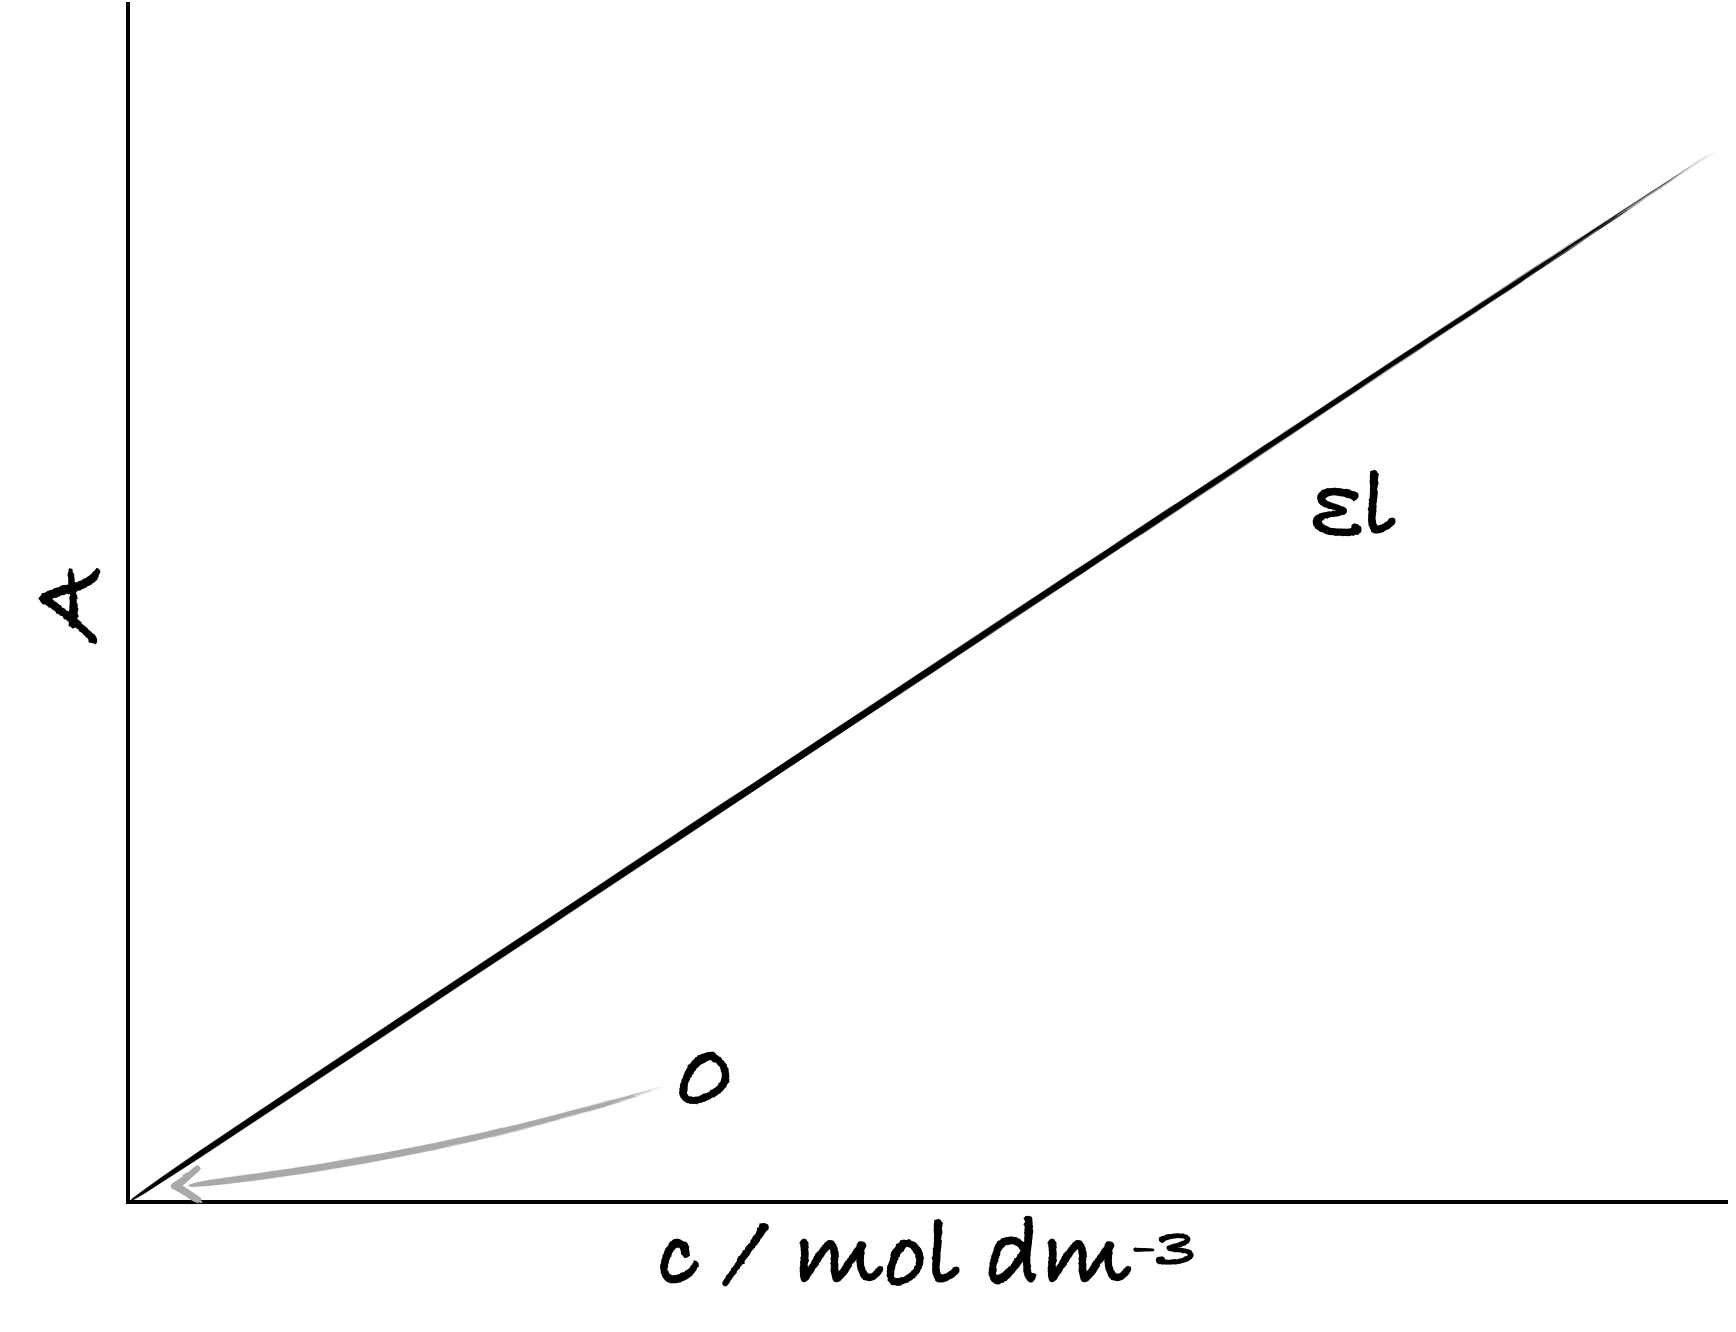
\includegraphics[width=0.3\linewidth]{images/abssketch} 

}

\caption{The Beer-Lambert relationship to show how absorbance, the dependent variable, changes with concentration, the independent variable.}\label{fig:abs}
\end{figure}

\begin{enumerate}
\def\labelenumi{\arabic{enumi}.}
\setcounter{enumi}{1}
\item
\end{enumerate}

\begin{figure}

{\centering 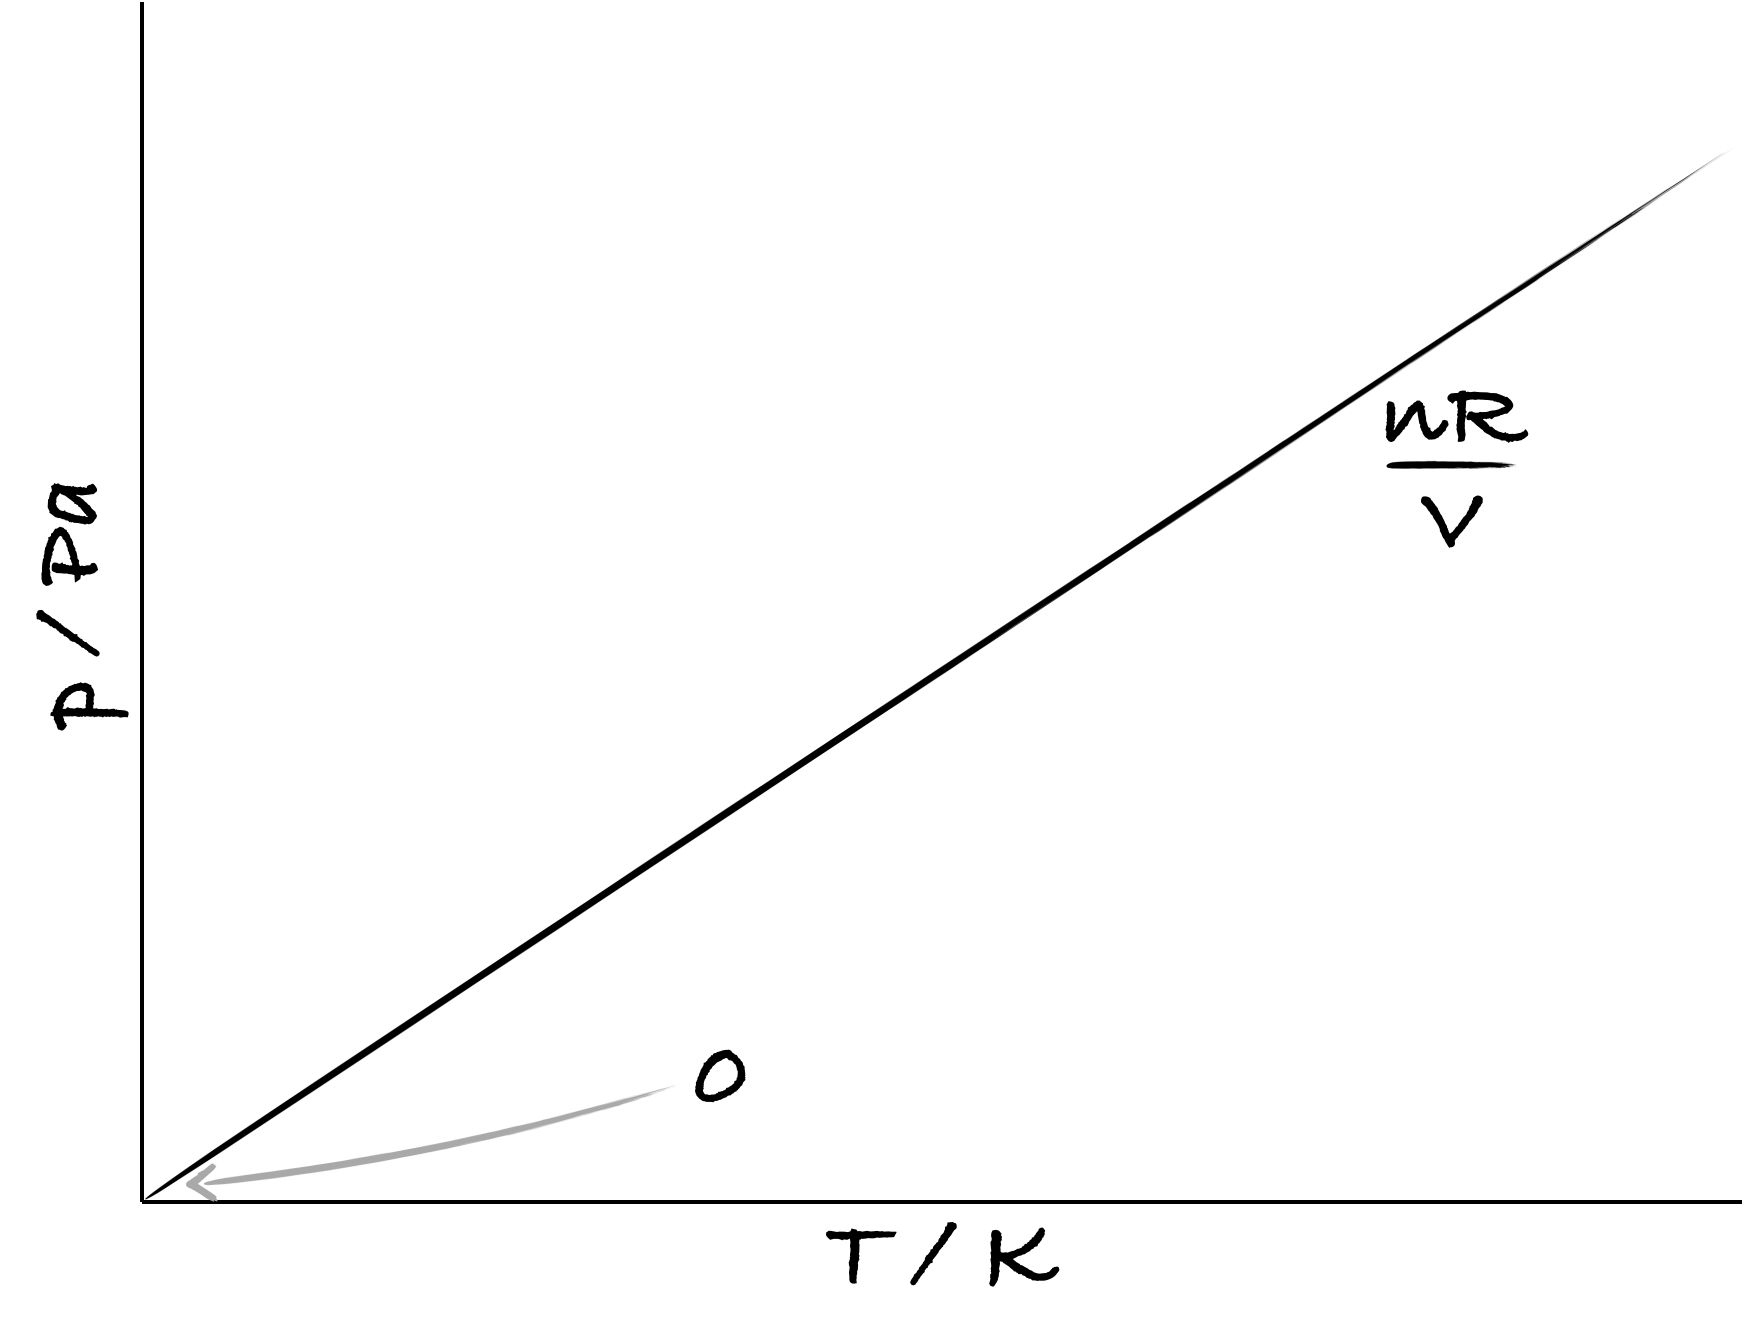
\includegraphics[width=0.3\linewidth]{images/pTsketch} 

}

\caption{A sketch to show how the pressure of an ideal gas, the dependent variable,changes with temperature, the independent variable.}\label{fig:pT}
\end{figure}

\begin{enumerate}
\def\labelenumi{\arabic{enumi}.}
\setcounter{enumi}{2}
\item
\end{enumerate}

\begin{figure}

{\centering 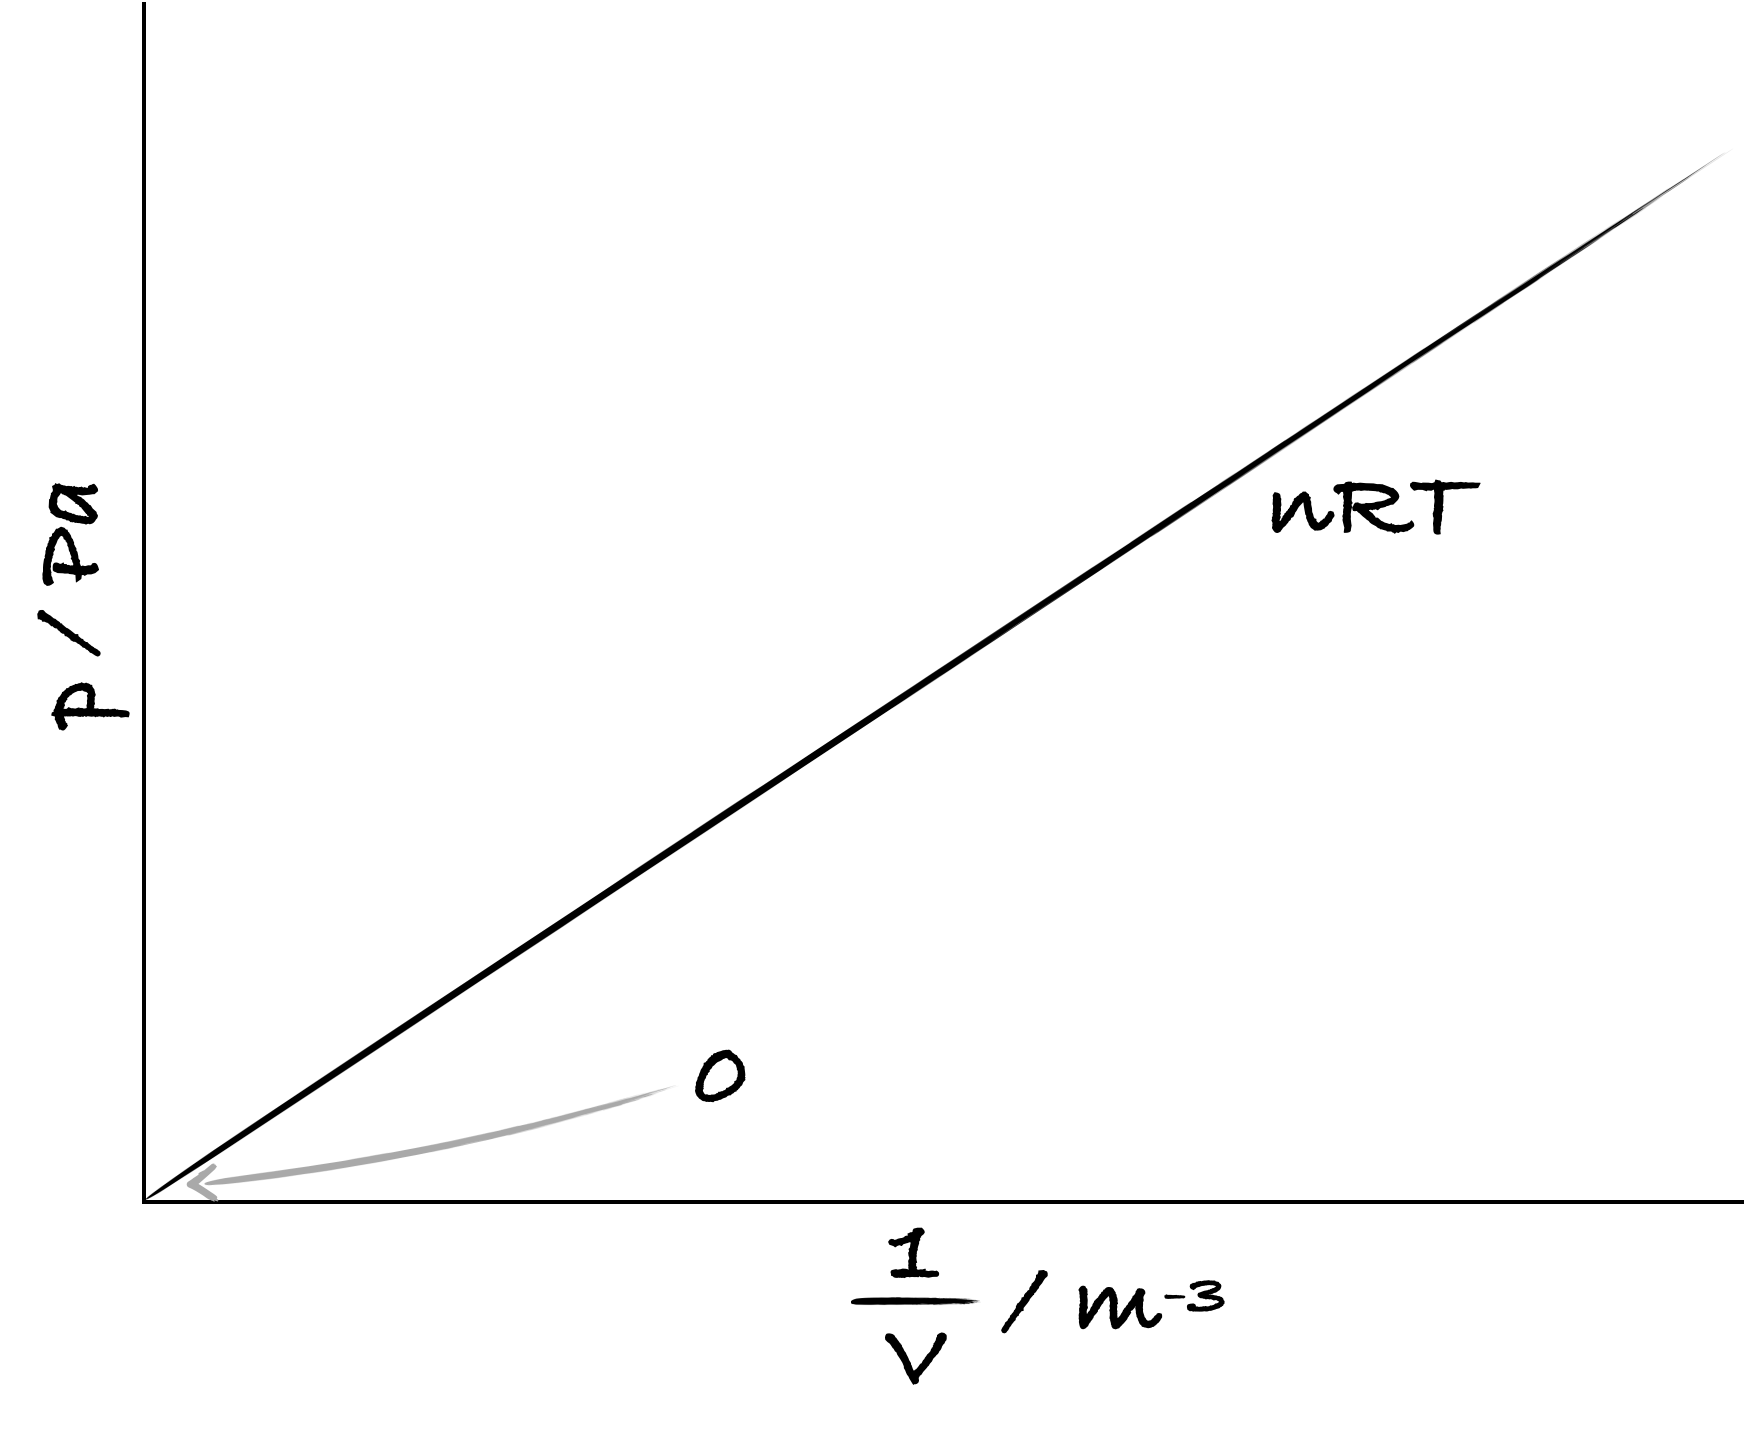
\includegraphics[width=0.3\linewidth]{images/pVsketch} 

}

\caption{A sketch to show how the pressure of an ideal gas, the dependent variable,changes with volume, the independent variable - note for a linear relationship we have 1/V on the x-axis.}\label{fig:pV}
\end{figure}

\hypertarget{subsec:2ndkinteticsans}{%
\subsection{Second order kinetics}\label{subsec:2ndkinteticsans}}

m = 3.19 M\textsuperscript{-1} s\textsuperscript{-1}, c = 180 M\textsuperscript{-1} ({[}A{]}\textsubscript{0} = 5.56 mM)

\hypertarget{subsec:clausiusans}{%
\subsection{Clausius-Clapeyron equation}\label{subsec:clausiusans}}

\(\Delta _{vap}H^\circ\) = 19.1 kJ mol\textsuperscript{-1}, 39 ºC.

\hypertarget{subsec:arrheniusans}{%
\subsection{Arrhenius equation}\label{subsec:arrheniusans}}

m = -22.4 × 10\textsuperscript{3} K, c = 43.7, \(E_a\) = 186 kJ mol\textsuperscript{-1}, \(A\) = 9.7 × 10\textsuperscript{18} s\^{}-1

  \bibliography{book.bib,packages.bib}

\end{document}
